\section{Análise de sentimento como processo de complementação}

Com a análise prévia dos textos fornecidos no \textit{dataset} e com o conhecimento prévio da plataforma \textit{Reddit}, foi observado que os textos têm alguma complexidade e variância no que toca à formalidade do mesmo.
Para facilitar a compreensão de um determinado texto, foi usado um modelo pré-treinado capaz de qualificar um texto em positivo, negativo e neutro. O modelo usado foi disponibilizado pelo grupo \textit{VADER Sentiment Analysis} \cite{vader}.

Como esta etapa foi usada como processo de complementação, este modelo foi aplicado a todos os textos do \textit{dataset}, com objectivo de mapear um valor capaz de qualificar o sentimento dos textos. Ou seja, o modelo possui como dados de entrada as matrizes transformadas no processo descrito na secção de pré-processamento e um valor que transmite o sentimento do texto.

Para efeitos de aprovação, o gráfico \ref{diagram:Sentiment_vs_no_sentiments} apresenta os valores da \textit{accuracy} do mesmo modelo com e sem a \textit{feature} que transmite o sentimento do texto. Como se pode observar, o modelo que dispunha da indicação do sentimento de texto obteve uma melhor performance em termos de \textit{accuracy} em ambos os conjuntos, o que indica que este valor é uma boa adição para a performance do modelo, já que ajuda a descodificar a parte semântica do texto que não é observável apenas com a noção de \textit{tokens}.


\begin{figure}[!t]
\begin{center}
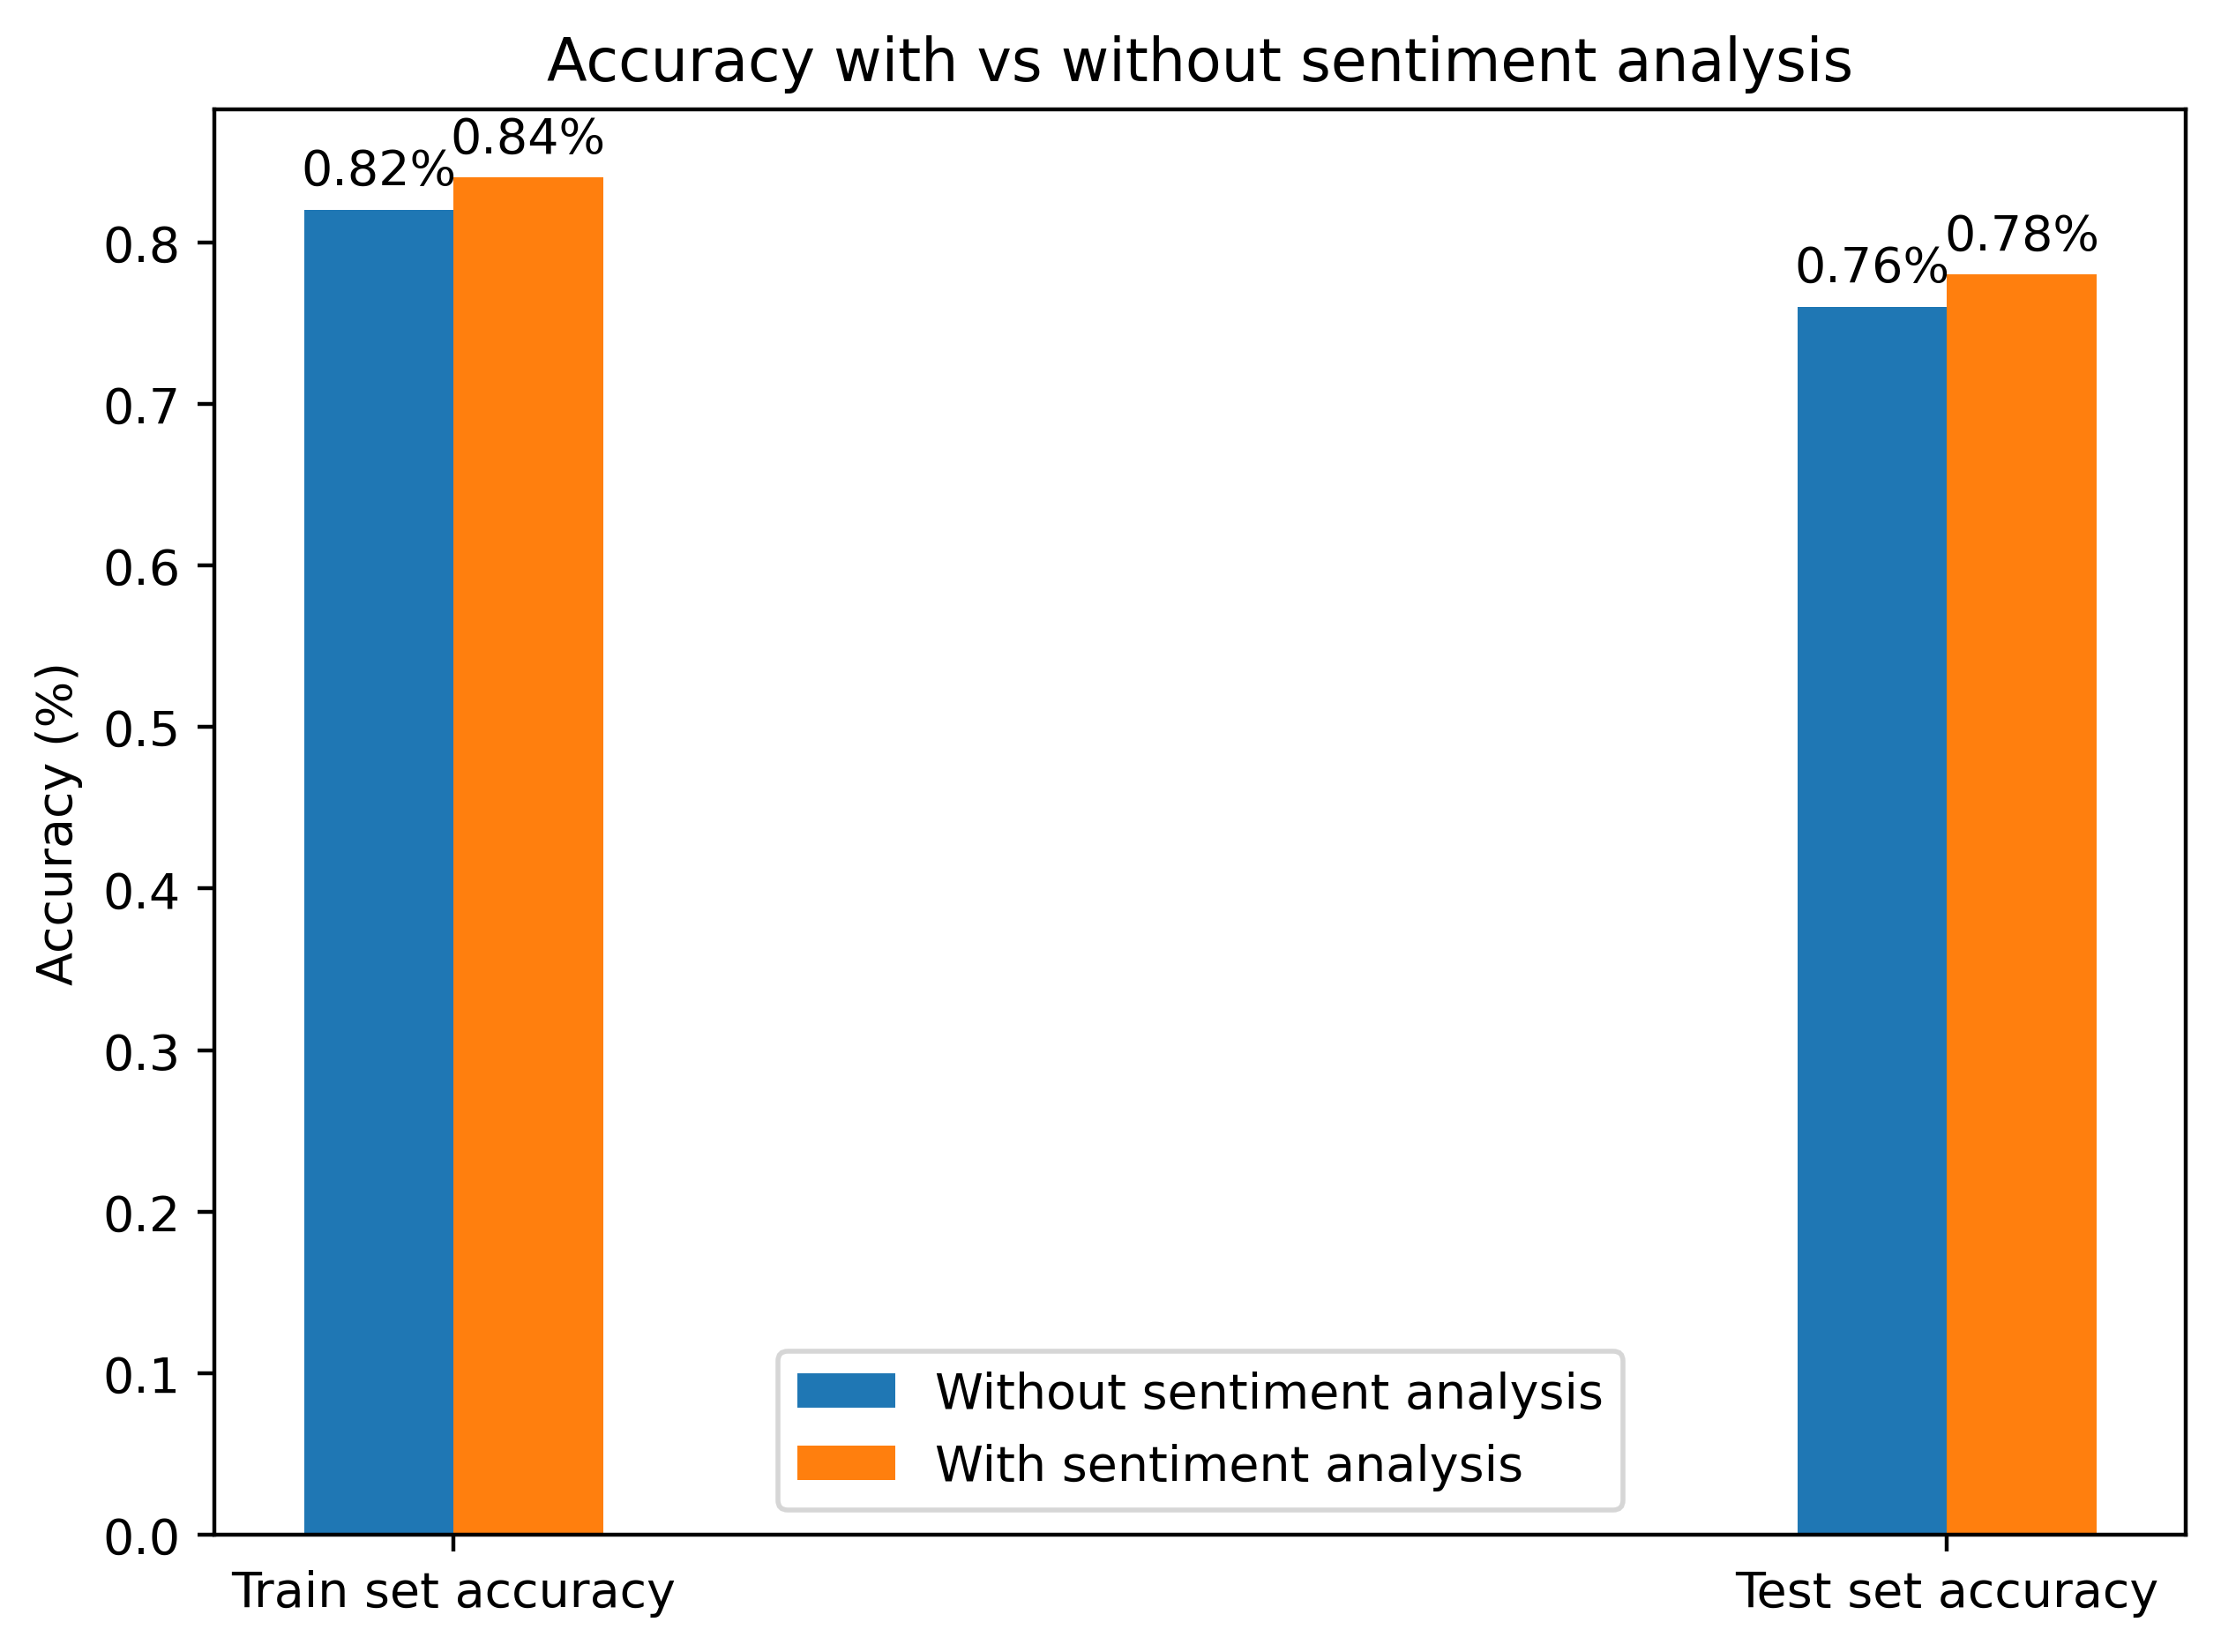
\includegraphics[width=0.5\textwidth,keepaspectratio]{figures/sentiment_vs_no_sentiment.png}
\caption{\textit{Accuracy} do mesmo modelo \textbf{com e sem} o valor que transmite o sentimento do texto}
\label{diagram:Sentiment_vs_no_sentiments}
\centering
\end{center}
\end{figure}
